\documentclass[compress]{beamer}
\mode<presentation>
{
 \usetheme{Vilanova}
}

\usepackage[french]{babel}

\usepackage[utf8]{inputenc}

\usepackage{times}
\usepackage[T1]{fontenc}

\usepackage{amsfonts}
\usepackage{amsmath}
\usepackage{amssymb}
\usepackage{tikz}
\usepackage{eurosym}
%\usepackage{url}
\usepackage[normal]{subfigure}
\newcommand{\goodgap}{%
	\hspace{\subfigtopskip}%
	\hspace{\subfigbottomskip}}



%\newtheorem{definition}{Definition}

\title{Corrections radiométriques}

\subtitle{Etalonnage et corrections atmosphériques} % (optional)


\author
{jordi.inglada@cesbio.cnes.fr}
\normalsize

\institute[Cesbio] % (optional, but mostly needed)
{\textsc{Centre d'Études Spatiales de la Biosphère, Toulouse, France}}

\date{}

\pgfdeclareimage[height=96mm,width=128mm]{background}{fondsClairSansLogo}
\setbeamertemplate{background}{\pgfuseimage{background}}
\pgfdeclareimage[height=0.6cm]{logoIncrust}{logoIncrust}
\pgfdeclareimage[height=0.5cm]{logo_cesbio}{logo_cesbio}
\logo{
\begin{tabular}{lp{0.25\textwidth}lp{0.25\textwidth}r}
\href{http://www.cesbio.ups-tlse.fr/}{\pgfuseimage{logo_cesbio}}
&&\footnotesize{AUF - Marrakech 2011}&&
\href{http://www.orfeo-toolbox.org}{\pgfuseimage{logoIncrust}}\\
\end{tabular}
}


\subject{Image radiometry in ORFEO Toolbox}




% Delete this, if you do not want the table of contents to pop up at
% the beginning of each subsection:
\AtBeginSubsection[]
{
  \begin{frame}<beamer>
    \frametitle{Outline}
    \tableofcontents[currentsection,currentsubsection]
  \end{frame}
}




% If you wish to uncover everything in a step-wise fashion, uncomment
% the following command: 

%\beamerdefaultoverlayspecification{<+->}
\begin{document}

\begin{frame}
  \titlepage
  \begin{center}
{\tiny Ce contenu est dérivé de la formation \href{http://www.orfeo-toolbox.org/packages/PragmaticRemoteSensing-handout.pdf}{``Pragmatic Remote
  Sensing''} dispensée par J. Inglada et E. Christophe en juillet 2010
  dans le cadre du colloque IGARSS. Il est mis à disposition selon les termes de la licence :\\
Creative Commons Paternité – Partage à l’Identique 3.0 non transcrit.} \href{http://creativecommons.org/licenses/by-sa/3.0/}{
\includegraphics[width=0.05\textwidth]{/home/inglada/Dev/GH/IGARSS2010/Tutorial/Slides/Ressources/CC-licence.png}}    
  \end{center}
\end{frame}

\section*{Introduction}

\begin{frame}

  \frametitle{Introduction}
  \begin{block}{Objectifs}
   \begin{itemize}
   \item Obtenir des mesures physiques à partir des images
   \end{itemize}
  \end{block}
  \begin{block}{6S}
   \begin{itemize}
    \item Nour utilisons le code de transfert radiatif : http://6s.ltdri.org/
    \item Code bien testé et validé
    \item Traduit automatiquement de Fortran à C
    \item Encapsulation transparente dans l'OTB
   \end{itemize}
  \end{block}

\end{frame}

\section{Corrections radiométriques}
\begin{frame}

  \frametitle{Les corrections radiométriques en 4 étapes}



\begin{center}
\begin{tikzpicture}[scale=0.18]
   \tiny

    \draw[->,thick] (0,0) --  +(3,0);
%     \pause

    \draw[fill=black!30,rounded corners=2pt] (4,-2) rectangle +(6,4);
    \node[text width= 0.8cm] (SensorModel) at (7,0) {CN vers Lum};
%     \pause

    \draw[->,thick] (11,0) --  +(3,0);
%     \pause

    \draw[fill=black!30,rounded corners=2pt] (16,-2) rectangle +(6,4);
    \node[text width= 0.85cm] (SensorModel) at (19,0) {Lum vers Réfl};
%     \pause


    \draw[->,thick] (23,0) --  +(3,0);
%     \pause

    \draw[fill=black!30,rounded corners=2pt] (27,-2) rectangle +(6,4);
    \node[text width= 0.85cm] (SensorModel) at (30,0) {TOA vers TOC};
%     \pause

    \draw[->,thick] (34,0) --  +(3,0);
%     \pause

    \draw[fill=black!30,rounded corners=2pt] (38,-2) rectangle +(6.5,4);
    \node[text width= 0.85cm] (SensorModel) at (41,0) {Adjacence};
%     \pause

    \draw[->,thick] (45,0) --  +(3,0);

 \end{tikzpicture}
\end{center}

  \begin{block}{Enchainement de filtres}
  Compatible avec la notion de {\em pipeline} de l'OTB
  \end{block}

\end{frame}

\subsection[CN vers Lum]{Du compte numérique vers la luminance}


\begin{frame}

  \frametitle{Du compte numérique vers la luminance}
     \begin{columns}

   \column{0.7\textwidth}
  \begin{block}{Objectif}
   \begin{itemize}
    \item Transformation du comte numérique en luminance
   \end{itemize}
  \end{block}
  Utilisation de otb::ImageToLuminanceImageFilter

  filterImageToLuminance->SetAlpha(alpha);

  filterImageToLuminance->SetBeta(beta);

  \column{0.3\textwidth}
  \footnotesize
  \begin{equation*}
   \mathbf{L_{TOA}^{k}} = \frac{ X^{k} } { \alpha_{k} } + \beta_{k}
  \end{equation*}
  \begin{itemize}
  \item $\mathbf{L_{TOA}^{k}}$ est la luminance incidente (en
  $W.m^{-2}.sr^{-1}.\mu m^{-1}$)
  \item $\mathbf{X^{k}}$  comte numérique
  \item $\alpha_{k}$ gain d'étalonnage pour la bande k
  \item $\beta_{k}$ biais d'étalonnage pour la bande k
  \end{itemize}

  \end{columns}
\end{frame}

\begin{frame}[fragile]
  \frametitle{Comment obtenir ces paramètres?}
  \begin{block}{Méta-données}
   \begin{itemize}
    \footnotesize
    \item Ces informations accompagnent souvent les images\ldots
    \item Mais le format des fichiers doit être connu!
   \end{itemize}
  \end{block}
  \begin{block}{A partir d'un fichier ASCII, ou à la main}
  \footnotesize
  \begin{verbatim}
  VectorType alpha(nbOfComponent);
  alpha.Fill(0);
  std::ifstream fin;
  fin.open(filename);
  double dalpha(0.);
  for( unsigned int i=0 ; i < nbOfComponent ; i++)
  {
      fin >> dalpha;
      alpha[i] = dalpha;
  }
  fin.close();
  \end{verbatim}
  \end{block}
\end{frame}

\subsection[Lum vers Réf]{De la luminance vers la réflectance}

\begin{frame}

  \frametitle{De la luminance vers la réflectance}
     \begin{columns}

   \column{0.6\textwidth}
  \begin{block}{Objectif}
   \begin{itemize}
    \item Transformer la luminance en réflectance
   \end{itemize}
  \end{block}
  \tiny
  Utilisation de otb::LuminanceToReflectanceImageFilter

  \texttt{filterLumToRef-> SetZenithalSolarAngle(zenithSolar);}

  \texttt{filterLumToRef-> SetDay(day);}

  \texttt{filterLumToRef-> SetMonth(month);}

  \texttt{filterLumToRef-> SetSolarIllumination(solarIllumination);}

  \column{0.3\textwidth}
  \footnotesize
  \begin{equation*}
   \rho_{TOA}^{k} = \frac{ \pi.\mathbf{L_{TOA}^{k}} } { E_{S}^{k}.cos(\theta_{S}).d/d_{0} }
  \end{equation*}
  \begin{itemize}
\tiny
  \item $\mathbf{rho_{TOA}^{k}}$ réflectance
  \item $\theta_{S}$ angle solaire zénital
  \item $E_{S}^{k}$ éclairement solaire au sommet de l'atmosphère à
    une distance $d_{0}$ de la Terre
  \item $d/d_{0}$ rapport entre la distance Terre-Soleil au moment de
    l'acquisition par rapport à la moyenne
  \end{itemize}

  \end{columns}
\end{frame}


\subsection{ToA vers ToC}




\begin{frame}

  \frametitle{Du sommet de l'atmosphère au sol}

  \begin{block}{Objectif}
   \begin{itemize}
    \item Corriger les effets atmosphériques
   \end{itemize}
  \end{block}
 
  
  \begin{columns}
  \column{0.5\textwidth}
  \footnotesize
  \begin{equation*}
   \rho_{S}^{unif} = \frac{ \mathbf{A} }{ 1 + Sx\mathbf{A} }
  \end{equation*}
  \column{0.5\textwidth}
  \begin{equation*}
   \mathbf{A} = \frac{ \rho_{TOA} - \rho_{atm} }{ T(\mu_{S}).T(\mu_{V}).t_{g}^{all gas} }
  \end{equation*}
  \end{columns}
  \begin{itemize}
  \item $\rho_{TOA}$ réflectance au sommet de l'atmosphère
  \item $\rho_{S}^{unif}$ réflectance au sol sous hypothèse de surface
    lambertienne et environnement uniforme
  \item $\rho_{atm}$ réflectance intrinsèque de l'atmosphère
  \item $t_{g}^{all gas}$ albédo sphérique
  \item $T(\mu_{S})$ transmittance vers le bas
  \item $T(\mu_{V})$ transmittance vers le haut
  \end{itemize}
\end{frame}

\begin{frame}

  \frametitle{Du sommet de l'atmosphère au sol}
  \begin{itemize}
  \tiny
  \item Utilisation de \texttt{otb::ReflectanceToSurfaceReflectanceImageFilter}

  \texttt{filterToAtoToC->SetAtmosphericRadiativeTerms(correctionParameters);}

  \item \texttt{otb::AtmosphericCorrectionParametersTo6SAtmosphericRadiativeTerms} 

\texttt{parameters->SetSolarZenithalAngle();}

\texttt{parameters->SetSolarAzimutalAngle();}

\texttt{parameters->SetViewingZenithalAngle();}

\texttt{parameters->SetViewingAzimutalAngle();}

\texttt{parameters->SetMonth();}

\texttt{parameters->SetDay();}

\texttt{parameters->SetAtmosphericPressure();}

\texttt{parameters->SetWaterVaporAmount();}

\texttt{parameters->SetOzoneAmount();}

\texttt{parameters->SetAerosolModel();}

\texttt{parameters->SetAerosolOptical();}
\end{itemize}
\end{frame}


\subsection{Effets d'adjacence}


\begin{frame}

  \frametitle{Effets d'adjacence}
     \begin{columns}

   \column{0.6\textwidth}
  \begin{block}{Objectif}
   \begin{itemize}
    \item Corriger les effets de voisinage
   \end{itemize}
  \end{block}

  \footnotesize
  Utilisation de \tiny \texttt{otb::SurfaceAdjacencyEffect6SCorrectionSchemeFilter}

  \footnotesize


  \tiny 
  \texttt{filterAdjacency->SetAtmosphericRadiativeTerms();}

  \texttt{filterAdjacency->SetZenithalViewingAngle();}

  \texttt{filterAdjacency->SetWindowRadius();}

  \texttt{filterAdjacency->SetPixelSpacingInKilometers();}

  \column{0.4\textwidth}
  \footnotesize
  \begin{equation*}
  \rho{S} = \frac{ \rho_{S}^{unif}.T(\mu_{V}) - <\rho{S}>.t_{d}(\mu_{v}) }{ exp(-\delta/\mu_{v}) }
  \end{equation*}
  \begin{itemize}
    \item $\rho_{S}^{unif}$ réflectance au sol sous hypothèse
      d'environnement uniforme
    \item $T(\mu_{V})$ transmittance vers le haut
    \item $t_{d}(\mu_{S})$ transmittance diffuse vers le haut
    \item $exp(-\delta/\mu_{v})$ transmittance directe vers le haut
    \item $\rho{S}$ proportion de la contribution de l'environnement à
      la réflectance du pixel observé
  \end{itemize}

  \end{columns}
\end{frame}

\subsection{Hands On}


\begin{frame}
\frametitle{Hands On}
\begin{enumerate}
\item Monteverdi: Calibration $\rightarrow$ Optical calibration
\item Select the image to correct
\item Look at the parameters that are retrieved from the image metadata
\item Apply the correction
\item Look at the different levels
\end{enumerate}
\end{frame}

\section{Pansharpening}

\begin{frame}
  \frametitle{Pansharpening}
  \framesubtitle{Bring radiometric information to high resolution image}
\centering
\begin{columns}
\begin{column}{0.45\textwidth}
 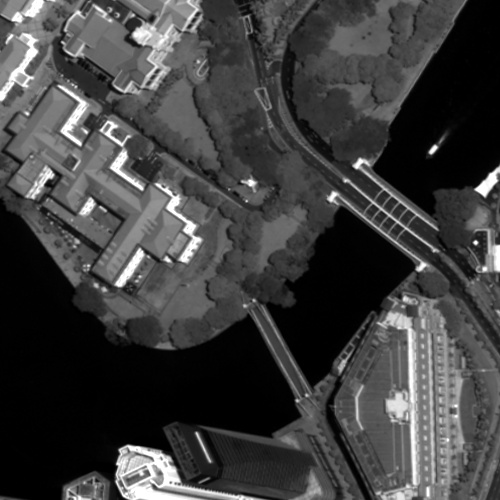
\includegraphics[width=0.6\textwidth]{panSharp-pan-extract.jpg}\\
 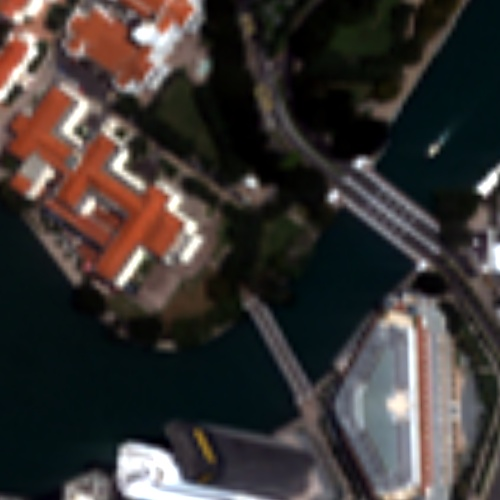
\includegraphics[width=0.6\textwidth]{panSharp-xs-extract.jpg}
\end{column}
%\begin{column}{0.10\textwidth}
%$\Rightarrow$
%\end{column}
\begin{column}{0.45\textwidth}
 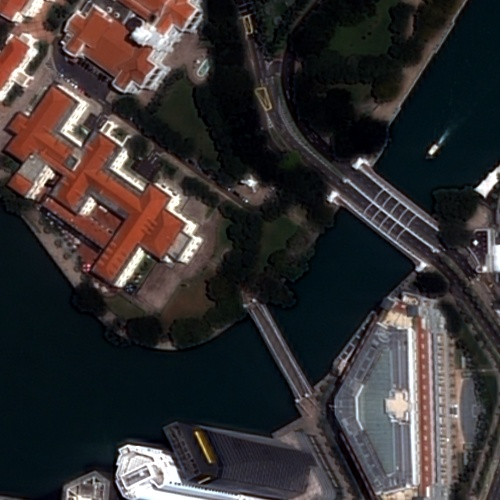
\includegraphics[width=0.6\textwidth]{panSharp-extract.jpg}
\end{column}
\end{columns}

\end{frame}

\begin{frame}
\frametitle{Hands On}
\begin{enumerate}
\item Monteverdi: Open two images, one PAN and one XS in the same geometry
\item Monteverdi: Filtering $\rightarrow$ Pan Sharpening
\end{enumerate}
\end{frame}

\end{document}
